\section{Model 3} 
As we just have seen, model 2 is constructed to have high curvature close to the sampled points only bounded by the small parameter $\delta>0$. The idea for the third model is to still have an inverse relation to the distance, but to bound the curvature in a more controlled way. It was Samson Seifu, a PhD student in our team who proposed the idea of the new distance dependent function, namely
\begin{equation*}
    f_3(d(\mathbf{x}; V)) = \frac{\sigma(\mathbf{x},t)}{\pi/2}\arctan(1/(\beta d(\mathbf{x}; V)))
\end{equation*} 
When $d\to 0$, $f_3(d) \to 1$, and thus there is no need for the parameter $\delta$ to avoid a singularity. The resulting model is thus

\begin{tcolorbox}[title=Model 3]
\begin{equation}
    u_t = |\nabla u| \bigg[ \frac{\alpha \sigma(\mathbf{x}, t)}{\pi/2} \tan^{-1}\bigg(\frac{1}{\beta \distanceVm}\bigg) + (1-\alpha)\kappa (u) \bigg], \quad \alpha, \beta \in \realspacem
    \label{eq:model3-pde}
\end{equation}
\end{tcolorbox}

Again, we do the same analysis on the radially symmetric example in order to get a feeling of how the curve, \curve\, will move following this model.

\subsection{Radially Symmetric Analysis}
We proceed in the in the same manner as for the two previous models. We rewrite the equation from $u(x, y)\to u(r)$ using \eqref{eq:curvature-circle} and \eqref{eq:nablau-ur}.
\begin{equation}
    u_t = u_r \, \bigg( \frac{\alpha \sigma(r, t)}{\pi/2} \tan^{-1}\bigg(\frac{1}{\beta |r-r_v|} \bigg) + \frac{1-\alpha}{r} \bigg).
    \label{eq:model3-rad}
\end{equation}
We can perform the same derivation as for model 1 and 2, deriving the ODE for the characteristics for the zero level curve, \curve:
\begin{equation}
    r_t = \frac{\alpha}{\pi/2} \tan^{-1}\bigg( \frac{1}{\beta(r(t)-r_v)}\bigg) + \frac{1-\alpha}{r(t)} \qquad \text{for } r(t)=\radgammam.
    \label{eq:model3-streamline-zero-levelcurve}
\end{equation}
Using \eqref{eq:sigma-radius-1} and \eqref{eq:sigma-radius-2} for the sign function $\sigma(r, t)$, we get the ODEs for all level curves:
\begin{alignat}{3}
    &r_t = - &(\alpha \tan^{-1}\big(\frac{1}{\beta|r(t)-r_v|} \big) + \frac{1-\alpha}{r(t)})  \qquad \text{when }&\radgammam\geq r_v, \\
    &r_t =  &(\alpha \tan^{-1}\big(\frac{1}{\beta|r(t)-r_v|} \big) - \frac{1-\alpha}{r(t)})  \qquad \text{when } &\radgammam< r_v.
\end{alignat}

Examples of such curves can be viewed in \figref{fig:total-streamline-arctan}. This shows the streamlines for zero level curves stemming from different initial radii. Here we can see that compared to model 2, the velocity near the point set is not as big, but increasing the value of $\beta$ yields a more similar shape for the streamline compared to model 2. However, since $\lim_{x\to\infty}\frac{2}{\pi} \arctan (x)=1$, the velocity will not be as high close to the sample points as model 1 with a small parameter $\delta$. 

\begin{figure}
    \begin{subfigure}{.5\linewidth}
        \centering
        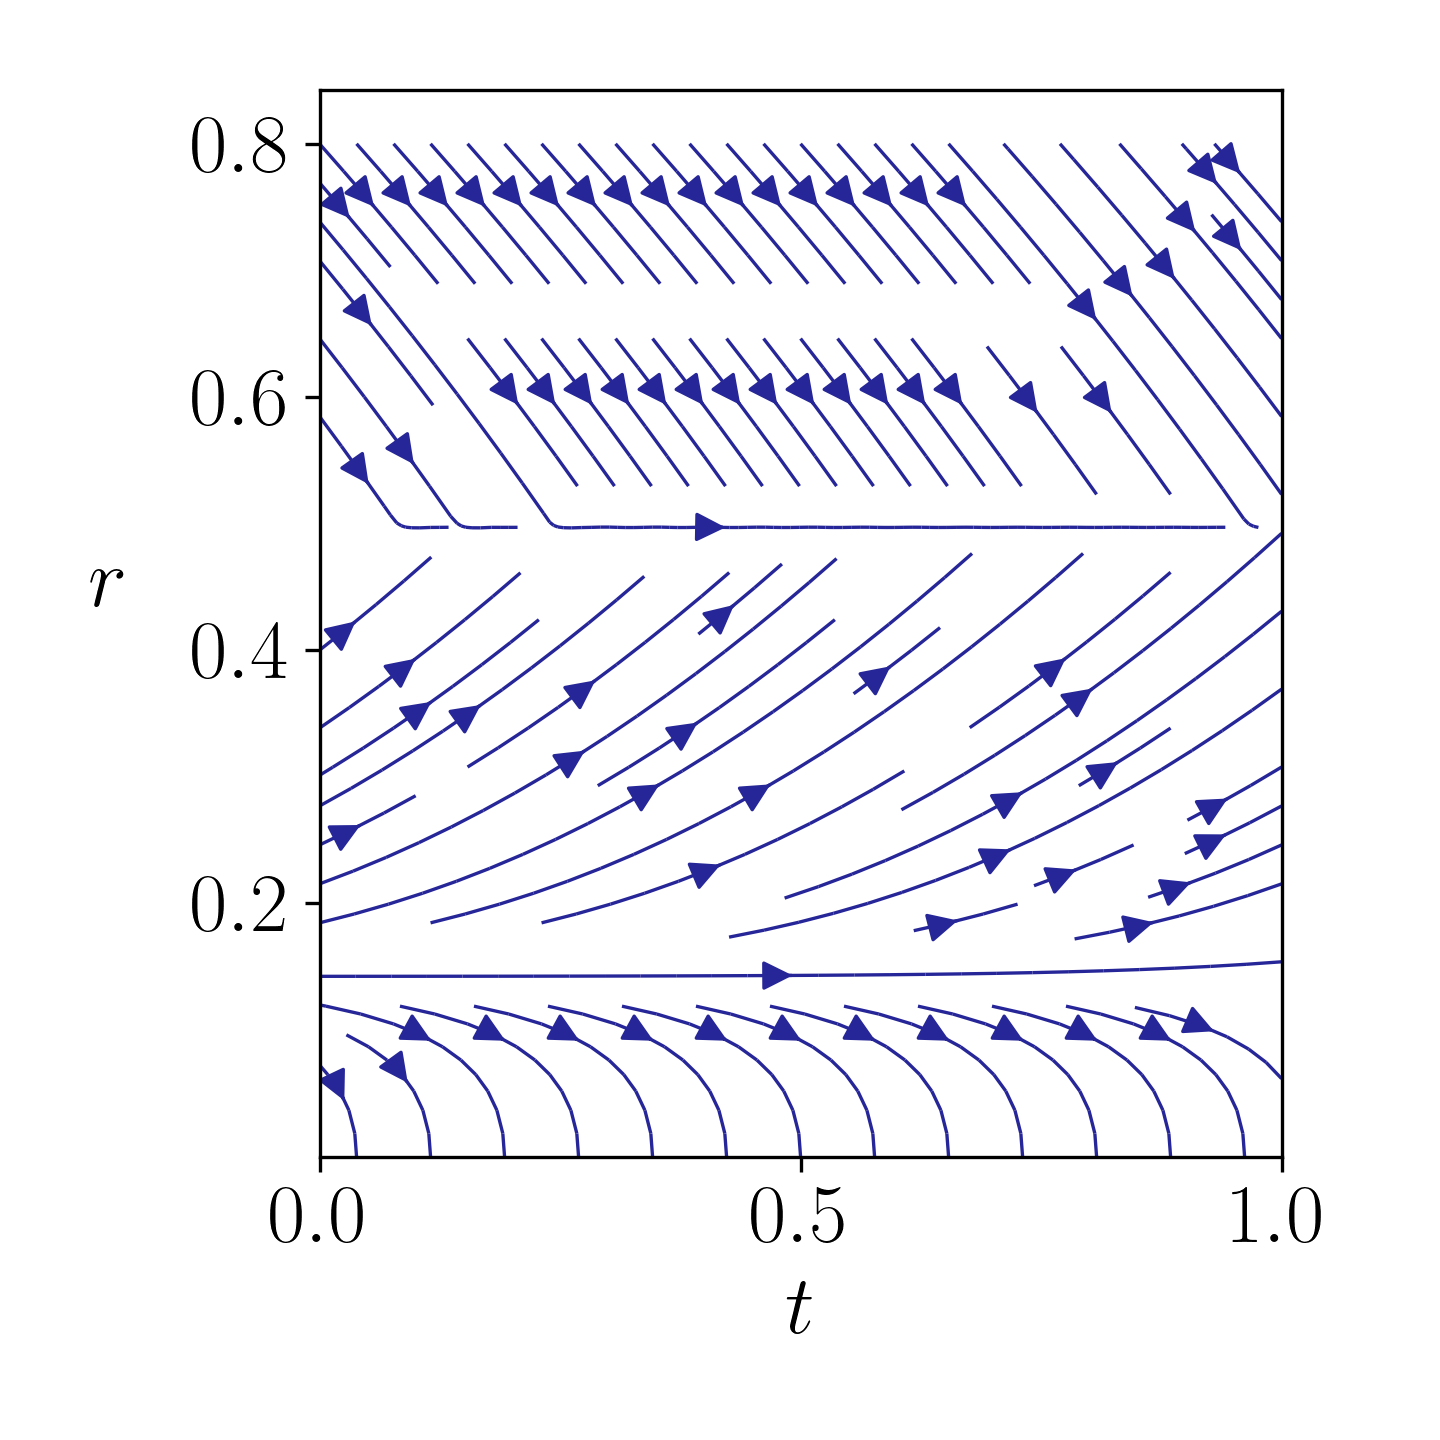
\includegraphics[width=\linewidth]{figures/streamlines/mod3-a90.png}
        \caption{$\beta=1$}
        \label{fig:arctan-sub1}
    \end{subfigure}%
    \begin{subfigure}{.5\linewidth}
        \centering
        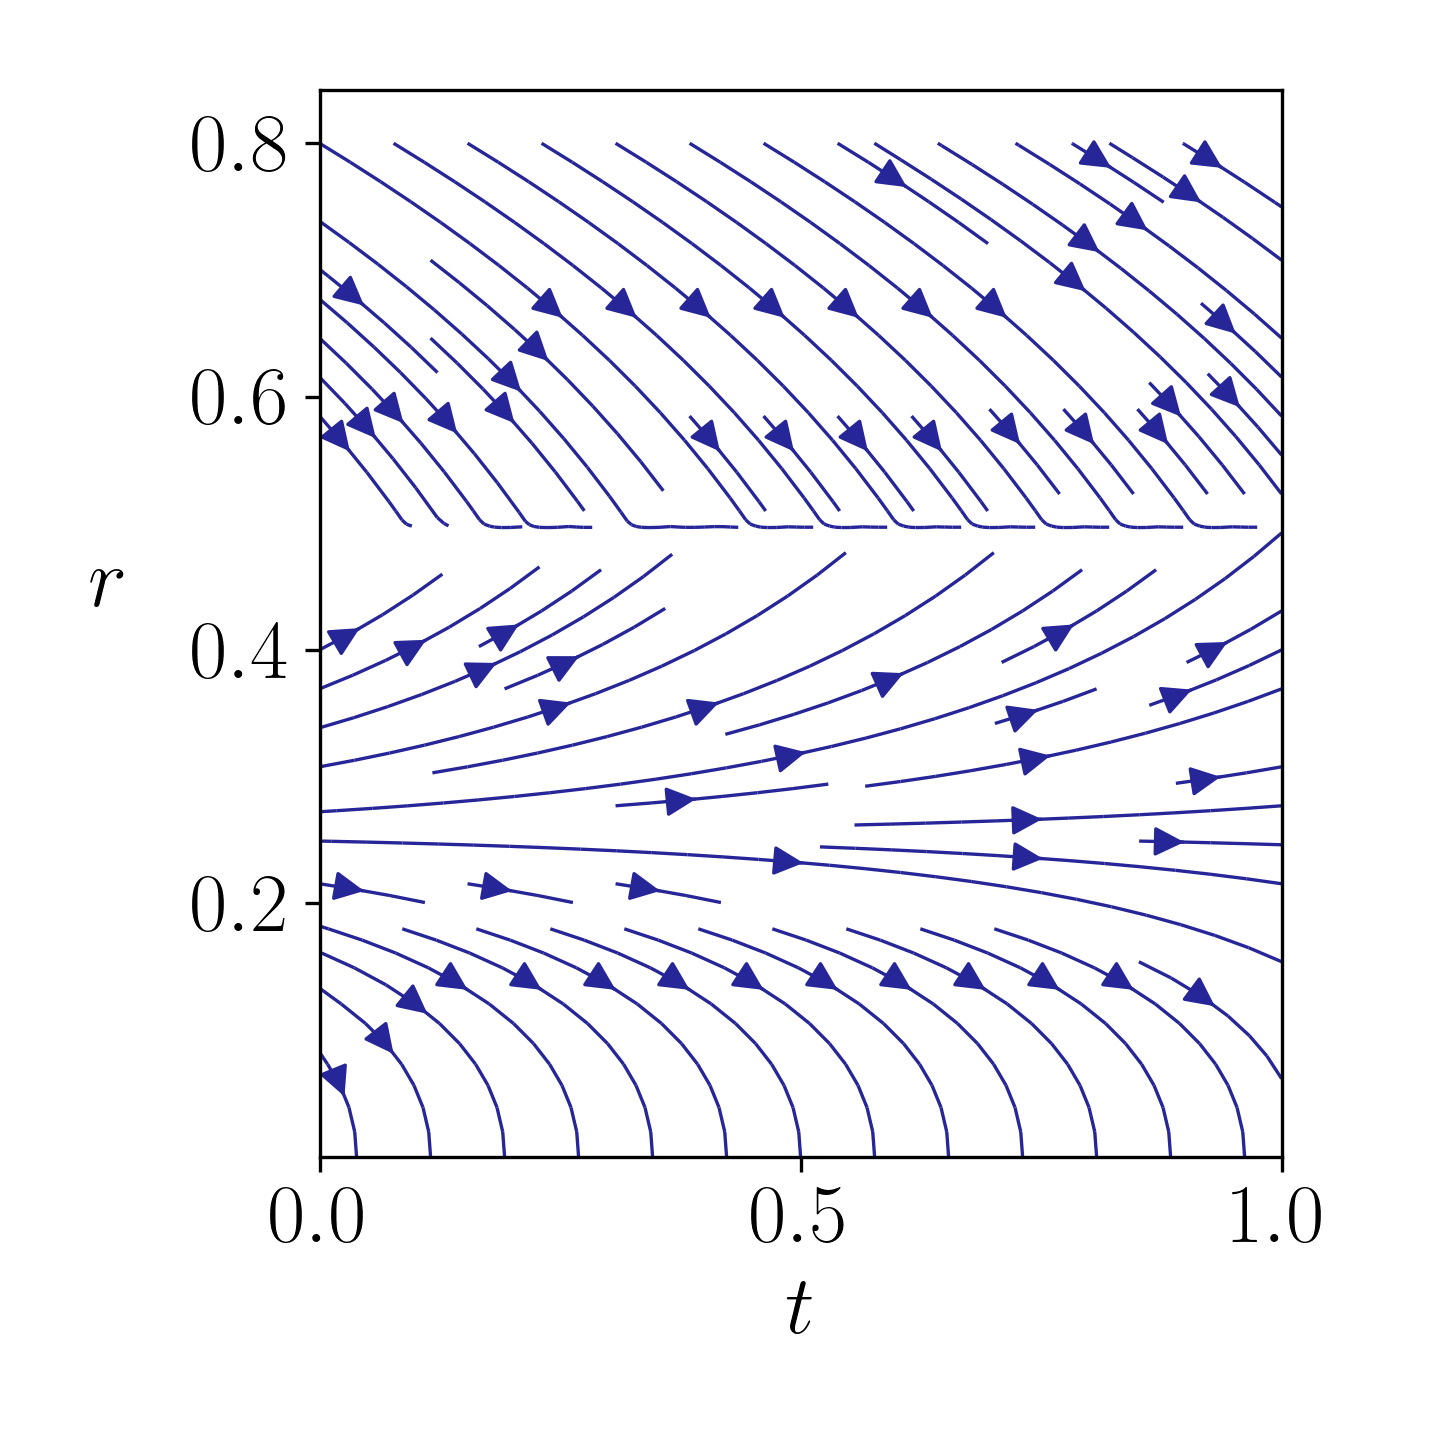
\includegraphics[width=\linewidth]{figures/streamlines/mod3-a90-b5.png}
        \caption{$\beta=5$}
        \label{fig:arctan-sub2}
    \end{subfigure}
    \caption[Streamlines for model 3]{Streamlines for the zero level set curve, $\Gamma(t)$, in the radially symmetric situation for model 3 defined in \eqref{eq:model3-pde} with the point set, \pointset, situated at $r_v=0.5$ and with parameter $\alpha=0.9$.}
    \label{fig:total-streamline-arctan}
\end{figure}

We move on to stationary solutions. As before, we are only interested in stationary solutions for the zero level curve, so we set $r_t$ from \eqref{eq:model3-streamline-zero-levelcurve} equal to zero.
We denote the stationary radius as $r_f$ and get \todo{Hva gjør jeg med dette???}
\begin{equation*}
    0 = \alpha \tan^{-1}\bigg( \frac{1}{\beta(r_f-r_v)} \bigg) + \frac{1-\alpha}{r_f}.
\end{equation*} 
\begin{comment}
After some simple operations, we obtain an implicit solution for the stationary radius,
\begin{equation}
    r_f-r_v = \bigg( \tan \bigg(\frac{1-\alpha}{\alpha r_f}\bigg) \bigg).
\end{equation}


\begin{enumerate}
    \item Curve stationary when covering the point set.
    \item Straight lines between, higher curvature close to points
    \item $\kappa(u) = \frac{\alpha}{1-\alpha} 2/\pi \arctan(1/d)$
\end{enumerate}
\end{comment}
\clearpage